\documentclass[hyperref={unicode}]{beamer}
\usepackage{CJKutf8}
\usepackage{color}
\usepackage{graphicx}
\usepackage{wrapfig}
\usepackage{hyperref}

\usetheme{Madrid}
%\usetheme{Warsaw}
%\usetheme{Singapore}
%\usetheme{Berlin}
\usecolortheme{whale}
% don't need for Madrid, but others need.
% \useoutertheme{infolines} 
% Adding footnotes
\usepackage{textpos} 
%\newenvironment{reference}[2]{% 
 % \begin{textblock*}{\textwidth}(#1,#2) 
  %    \footnotesize\it\bgroup\color{red!50!black}}{\egroup\end{textblock*}} 
% changing the itemization markers
\setbeamertemplate{items}[ball]

% Rounder boxes and shadows
\setbeamertemplate{blocks}[rounded][shadow=true]
% Getting rid of the nabigation icons
\setbeamertemplate{navigation symbols}{}

\begin{document}

\begin{CJK}{UTF8}{gkai}


\title{Save the Whales, Save the World}
%\subtitle{AI Course Presentation}
\author[StephenLee]{
\includegraphics[height=1cm, width=2cm]{logo}\\StephenLee\\(李晓东)}
% \date{\today}
\renewcommand{\today}{ April 24, 2012}
\institute[STW]{\alert{S}AVE \alert{T}HE \alert{W}HALES \alert{A}GAIN \\ A Whaleman Foundation International Campaign}

 \logo{
\includegraphics[width=1cm, height=1cm]{stwlogo}}

\begin{frame}
  \maketitle
\end{frame}

% automatically print the table of contents  at the beginning of each
% section and subsection.
\AtBeginSection[]
{
  \begin{frame}
    \tableofcontents[currentsection,currentsubsection]
  \end{frame}
}

\section{Whale Hunting}
\begin{frame}{Whale Hunting}
\begin{block}{With specific regards to whale hunting, the New York Times reported in 2010 that there are three countries in particular -- Japan, Norway, and Iceland -- that are key to any international consent to stop commercial whaling:}
\begin{itemize}
\item Right now, despite the world-wide moratorium on commericial whaling, Since 1986, Japan has defied the moratorium by killing thousands of whales under the guise of \alert{scientific research}.
\pause
\item Norway has also defied the commercial whaling moratorium, killing over \alert{500} minke whales per year as well. 
\end{itemize}
\end{block}
\end{frame}
\section{Whalers' Myths-and the Reality}
\begin{frame}{No.1: Whales eat too many fish and must be culled}
  \begin{block}{The statement is unscientific and has no basis in fact.}
    \begin{itemize}
    \item Many whales do not eat fish at all; indeed, most of the world's baleen whales live in the Southern Hemisphere, where they primarily eat krill.
      \pause
    \item The primary predators of fish are not whales, but other fish. The removal of top predators (such as cetaceans) can cause major ecosystem disturbances, with negative consequences for fisheries.
    \end{itemize}
  \end{block}
\end{frame}

\begin{frame}{No.2: Whale populations are numerous and increasing}
  \begin{block}{These arguments are based on some doubtful science}
    \begin{itemize}
    \item The website of Japan's Institute of Cetacean Research (ICR) claims that populations of humpback and fin whales are growing by 14-16 percent. The IWC's Scientific Committee has agreed is biologically impossible.
      \pause
    \item The Japanese government continues to cite an outdated estimate of 760,000 minke whales in the Southern Hemisphere.
    \end{itemize}
  \end{block}
\end{frame}
\begin{frame}{No.3: Commercial whaling is essential for traditional, cultural or nutritional}
  \begin{block}{Japan's whaling tradition dates back only a few centuries, Japan's Antarctic whaling did not begin until the 1930s.}
    \begin{itemize}
    \item The Icelandic government has made it clear that commercial whaling will only continue if an export market can be found.
      \pause
     \item Meanwhile, Japan has more than 4,000 tons of whale meat from its "scientific" whaling program in cold storage - uneaten, unsold, and unwanted.
    \end{itemize}
  \end{block}
\end{frame}

\section{Some numbers}
\begin{frame}{Endangered Whales}
  \begin{block}{Blue And Fin Whales}
    Over 1 million whales were slaughtered in the Antarctic last century, seriously depleting 7 of the 8 species of great whales found there. In 1989, the results of an IWC whale population survey in Antarctica revealed that blue and fin whales had been depleted by between \alert{95-99\%} from whaling. The blue whale population was reduced to fewer than \alert{1,000} from an estimated quarter-million animals. Blue whales were once the mainstay of the Antarctic whaling industry. Over \alert{30,000} were killed in a single season in 1931 and the species has never recovered.
  \end{block}
\end{frame}

\section{Join the fight}
\begin{frame}{It's time to stop this senseless slaughter now!!!}
\begin{itemize}
\item Write, e-mail, or call \alert{President Obama} and thank him for taking action against Iceland and let him know that you want the US to use its sanctioning powers available under the Pelly Amendment against Japan and Norway as well until they stop whaling. His contact at: \alert{http://www.whitehouse.gov/contact/} 
\pause
\item Write the Japanese Prime Minister, \alert{Noda Yoshihiko}, and tell him you will not purchase any Japanese products or visit Japan until they stop killing and capturing dolphins and whales.
\pause
\item Do not \alert{participate} in any captive swim-with dolphin programs.
\pause
\item Do not support or \alert{visit} any marine park, zoo, or amusement park that has captive dolphins and whales.
\pause
\item \alert{Advice}:Dont't try to refer to Chinese's goverment. They are busy now, they won't cope with it.
\end{itemize}
\end{frame}
\begin{frame}{To be a hero}
\begin{columns}
\begin{column}{0.5\textwidth}
  \begin{center}
  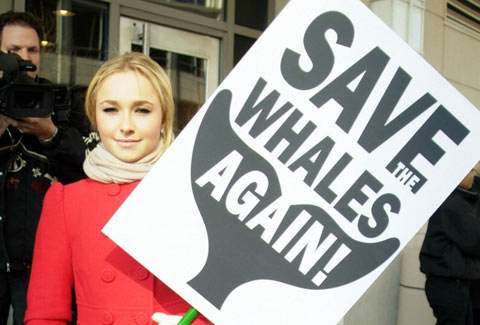
\includegraphics[width=0.8\textwidth]{save_the_whale}
  \end{center}
\end{column}

\begin{column}{0.5\textwidth}
  \begin{itemize}
  \item To forever preserver and protect whales and dolphins and their critical habitats.
    \pause
  \item To perform long-tem field research of cetaceans and their interrelationships with mankind in order to better understand the context of their lives for the betterment of all.
    \pause
\item To raise awareness to the issuss that not only affect cetaceans, but all marine life, and the overall health of our oceans.
  \pause
\item To share what we observe, learn and value with the world.
\end{itemize}
\end{column}
\end{columns}
\end{frame}

\section{The end}
\begin{frame}{Q\&A}
  \begin{center}
    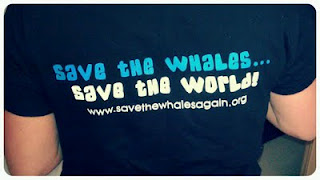
\includegraphics[width=7cm]{website} \\
    \LARGE{\alert{Thanks!}}
  \end{center}
\end{frame}
\end{CJK}
\end{document}

